\documentclass[11pt]{article}
\usepackage[margin=25mm]{geometry}
\usepackage{amsmath}
\usepackage{float}
\usepackage{subfig}
\usepackage{listings,color,enumitem}
\definecolor{mygreen}{RGB}{28,172,0} % color values Red, Green, Blue
\definecolor{mylilas}{RGB}{170,55,241}
\usepackage{graphicx}
\title{Problem Set 3\\ \vspace{2mm}\Large{16-642 Manipulation, Estimation, and Control}}
\author{Matthew Swenson \thanks{Worked with Karsh Tharyani}}
\begin{document}
	\maketitle
	
\section*{Question 1}
\subsection*{a}
The eigenvalues of the A matrix in the given system are 
$$
\gamma_i=
\left(\begin{array}{c} 7.669\\ -0.33449+0.13606{}\mathrm{i}\\ -0.33449-0.13606{}\mathrm{i} \end{array}\right)
$$
There is an eigenvalue with greater than zero real part, so the system is unstable.
\subsection*{b}
The matrix $$ Q =[A AB A^2B]=
    \left(\begin{array}{ccc} 1.0 & 0 & 0\\ 0 & 0 & 1.0\\ 0 & 1.0 & 7.0 \end{array}\right)$$
has rank = 3, so it is controllable.
\subsection*{c}
$$ W_o=\begin{bmatrix}C\\CA\\CA^2\end{bmatrix}=\left(\begin{array}{ccc} 0 & 1.0 & 3.0\\ 3.0 & 15.0 & 22.0\\ 22.0 & 113.0 & 169.0 \end{array}\right)$$
     The rank of $W_o$ is 3, so the system is observable.
\subsection*{d}
\begin{figure}[H]
    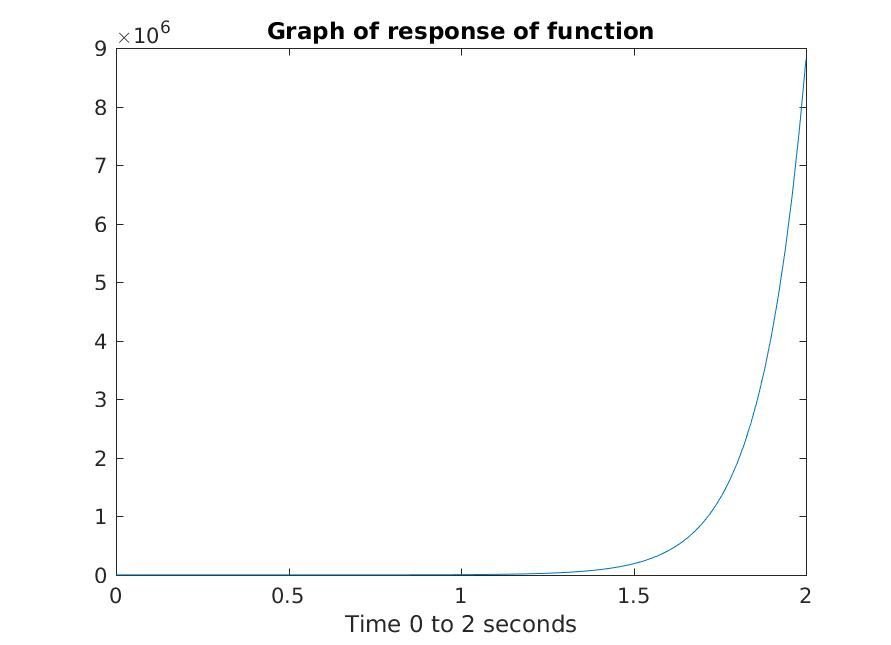
\includegraphics[width=.7\textwidth]{q1d.jpg}
\end{figure}
\subsection*{e}
    $$K=\left[\begin{array}{ccc} 11.0 & 60 & 88 \end{array}\right]$$
\subsection*{f}
\begin{figure}[H]
    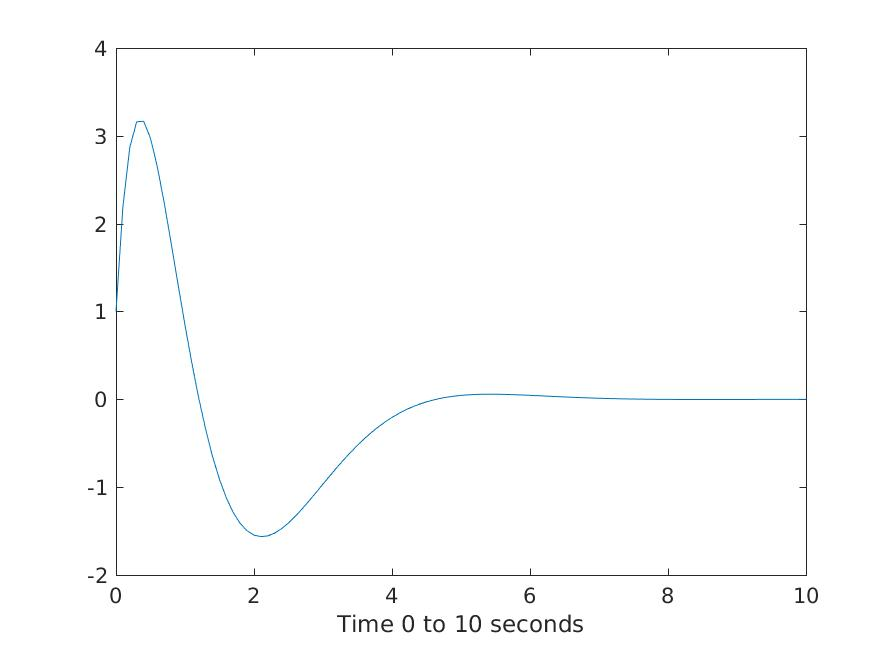
\includegraphics[width=.7\textwidth]{q1f.jpg}
\end{figure}
\section*{Question 2}
\subsection*{a}
Looking at the system, we can put it into standard mechanical form, with the following matricies:
$$
M = \left[\begin{array}{cc} \gamma & -\beta\,\cos\left(\varphi \right)\\ -\beta\
,\cos\left(\varphi \right) & \alpha  \end{array}\right]
$$
$$
C=\left[\begin{array}{cc} \mu  & \beta\,{x_{4}}^2\,\sin\left(\varphi \right)\\ 
        0 & 0 
\end{array}\right]
$$
$$
G=\left[\begin{array}{c} -F\\ -D\,\sin\left(\varphi \right) \end{array}\right)
$$
We can figure out the bottom two entries of $\dot{x}$ by solving for the acceleration term of the standard form. This yields:
$$
\begin{bmatrix}
    \ddot{x_1}\\
    \ddot{x_2}
\end{bmatrix}
=
M^{-1}\left[-C
\begin{bmatrix}
    \dot{x_1}\\
    \dot{x_2}
\end{bmatrix}
-F\right]
$$
Simplifying the bottom two terms and adding in the trivial $x_3$ and $x_4$, we get:
$$
\dot{x}=
\left[\begin{array}{c}
        x_{3}\\ 
        x_{4}\\
        -\frac{-\alpha \,\beta\,\sin\left(\varphi \right)\,{x _{4}}^2+F\,\alpha -\alpha \,\mu \,x_{3}+D\,\beta\,\cos\left(\varphi \right)\,\sin\left(\varphi\right)}{\alpha \,\gamma-{\beta}^2\,{\cos\left(\varphi \right)}^2}\\
        -\frac{F\,\beta\,\cos\left(\varphi \right)+D\,\gamma\,\sin\left(\varphi \right)-\beta\,\mu \,x_{3}\,\cos\left(\varphi \right)-{\beta}^2\,{x_{4}}^2\,\cos\left(\varphi \right)\,\sin\left(\varphi \right) }{\alpha \,\gamma-{\beta}^2\,{\cos\left(\varphi \right)}^2}
\end{array}\right]
$$
\subsection*{b}
The equilibrium points of the system occur whenever the velocity terms and driving forces are zero. This causes the entire first equation to go to zero,
and the second to become $-D\sin{phi}=0$ Because $\sin$ is a cyclical function, there is an equilibrium point at $phi = \pi/2$ and every $\pi$ revolutions thereafter.
This corresponds to the arm of the pendulum being straight up or down.
\subsection*{c}
\begin{figure}[H]
   %\centering
 \begin{tabular}{cc}
    \subfloat[]{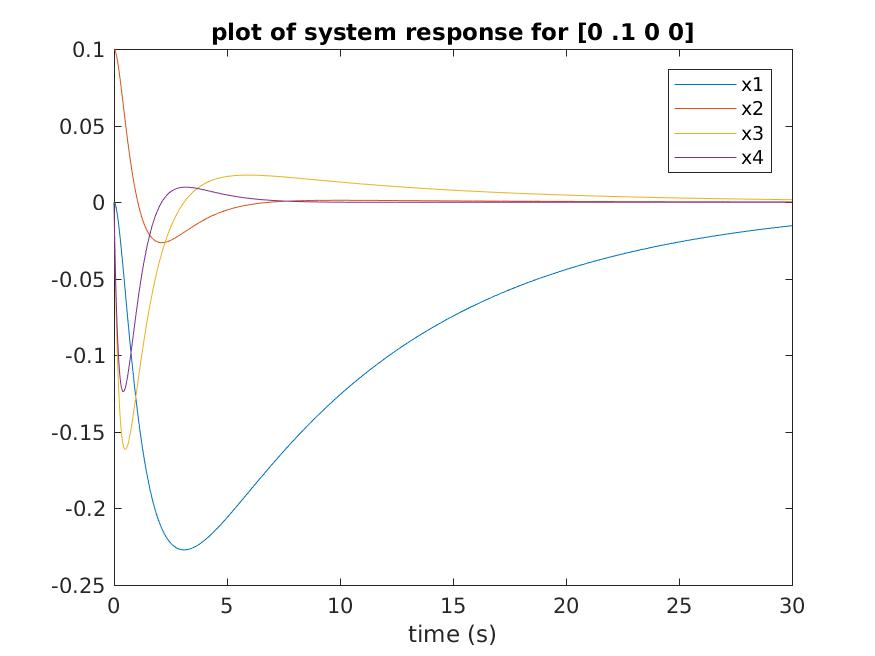
\includegraphics[width=.5\textwidth]{q2c1.jpg}} &
    \subfloat[]{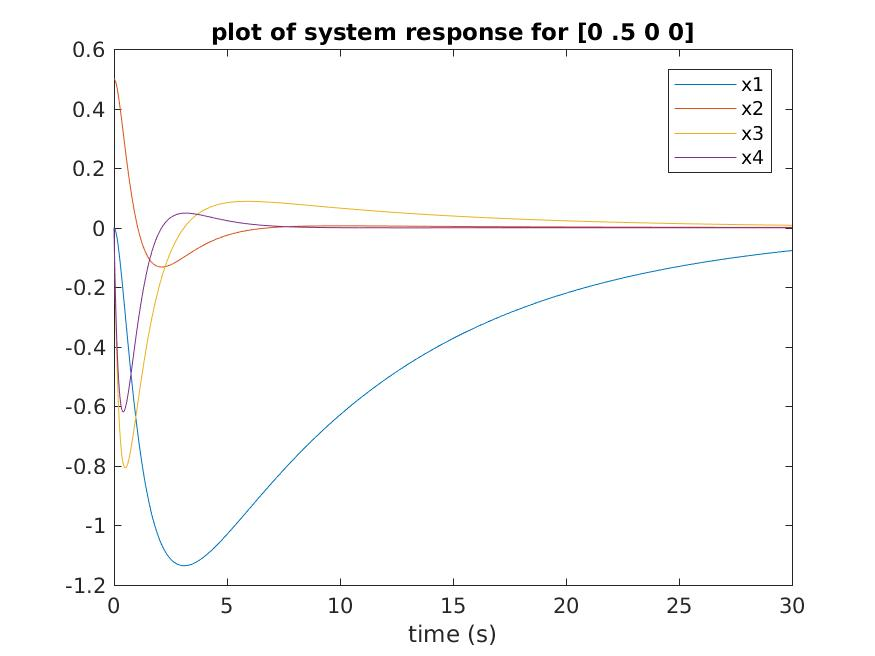
\includegraphics[width=.5\textwidth]{q2c2.jpg}} \\
    \subfloat[]{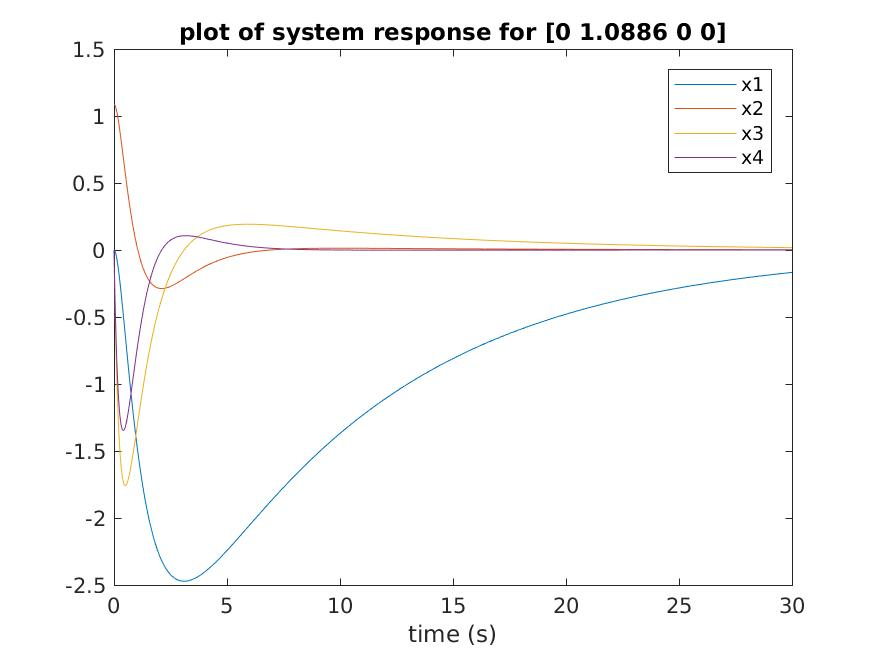
\includegraphics[width=.5\textwidth]{q2c3.jpg}} &
    \subfloat[]{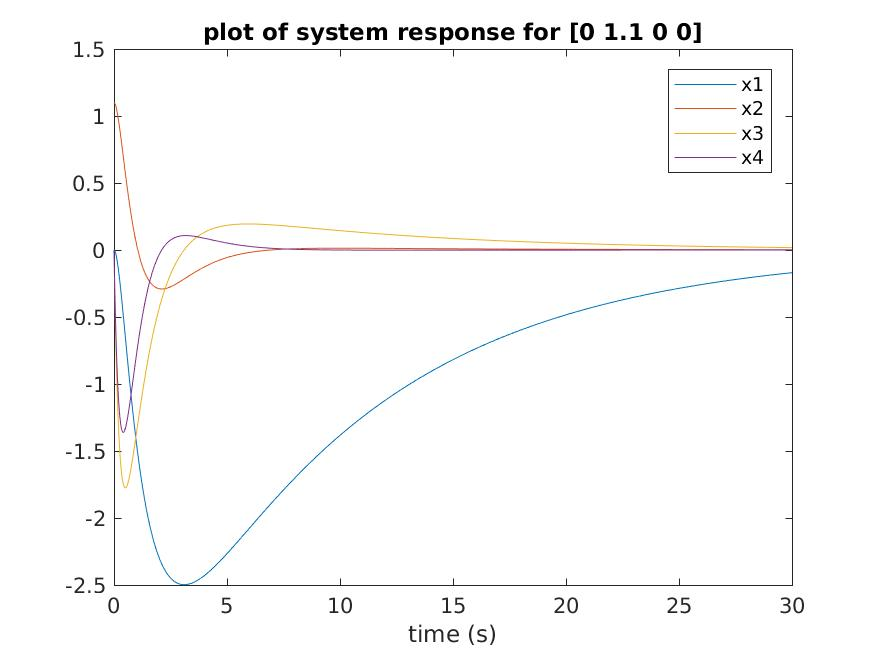
\includegraphics[width=.5\textwidth]{q2c4.jpg}} 
\end{tabular}
    \caption{Plots of the linearized system at various initial conditions. The shape of the response does not change, but the timescale does.}
\end{figure}

\subsection*{d}
\begin{figure}[H]
   %\centering
 \begin{tabular}{cc}
    \subfloat[]{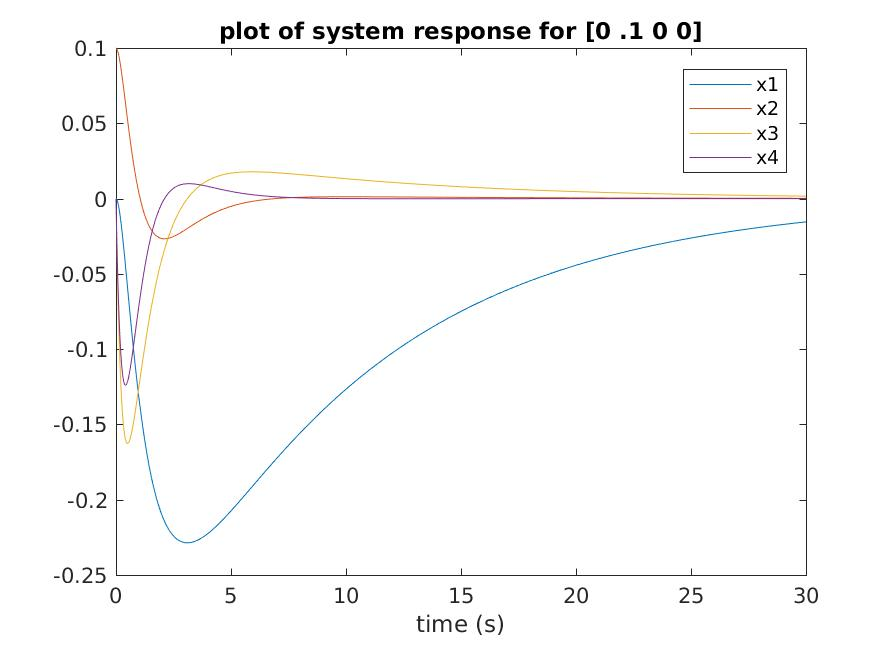
\includegraphics[width=.5\textwidth]{q2d1.jpg}} &
    \subfloat[]{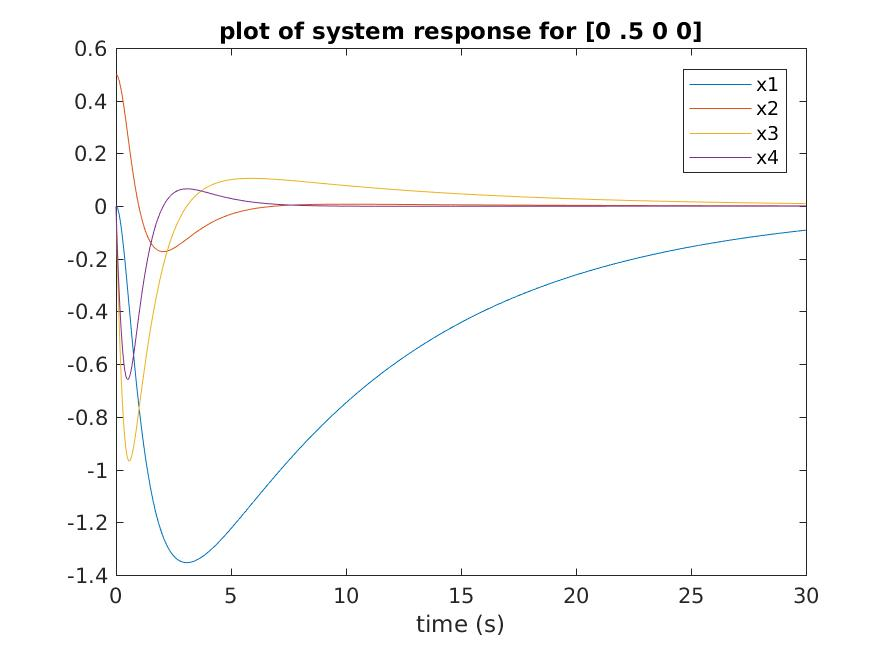
\includegraphics[width=.5\textwidth]{q2d2.jpg}} \\
    \subfloat[]{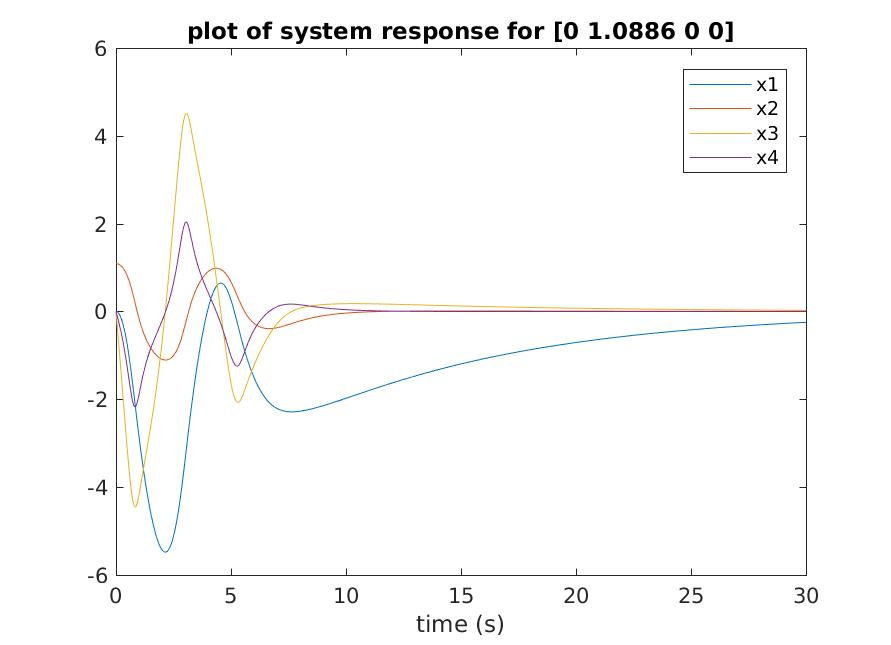
\includegraphics[width=.5\textwidth]{q2d3.jpg}} &
\end{tabular}
    \caption{Plots of the nonlinear system at various initial conditions. The behavior for the first to initial conditions is virtually identical,
             but the system becomes noticably more unstable for 1.0866 and does not converge for the 1.1 initial condition.}
\end{figure}
\section*{Question 3}
\subsection*{a}
The closed loop unity negative feedback function is $T=\frac{H}{H+1}$, so using matlab to define the transfer function, 
we get 
$$
T(s) = \frac{200 s^3 + 4400 s^2 + 28200 s + 400}
{s^6 + 44 s^5 + 766 s^4 + 6408 s^3 + 24369 s^2 + 28764 s + 404}
$$
\subsection*{b}
Using matlab, 
$$
poles =\left[\begin{array}{c} -10.993+4.4546{}\mathrm{i}\\ -10.993-4.4546{}\mathrm{i}\\ -10.0+1.0{}\mathrm{i}\\ -10.0-1.0{}\mathrm{i}\\ -2.0\\ -0.014216 \end{array}\right]
$$
$$
zeroes = \left[\begin{array}{c} -10.993+4.4546{}\mathrm{i}\\ -10.993-4.4546{}\mathrm{i}\\ -0.014216 \end{array}\right]
$$
\subsection*{c}
\begin{figure}[H]
    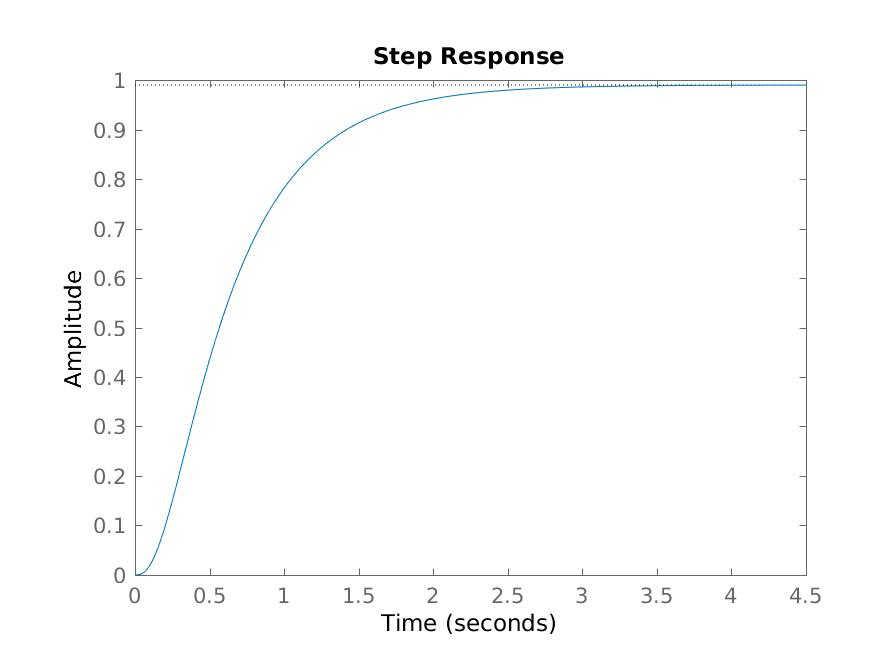
\includegraphics[width=.7\textwidth]{q3.jpg}
\end{figure}
The dominant pole is at -.014216, as demonstrated by its significantly smaller distance to the 
imaginary axis, and the overdamped response of the system.
\subsection*{d}
The final value theorem states that the steady state response of a system is the limit of the 
transfer function as $s$ approches zero. Setting $s = 0$ in the above gives $y_{ss}=\frac{400}{404}=0.9900990099$.

\section*{Question 4}
\begin{figure}[H]
    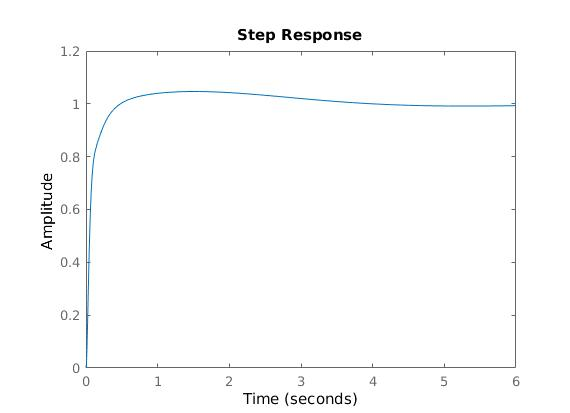
\includegraphics[width=.7\textwidth]{q4.jpg}
\end{figure}
The above figure was created with the following parameters:
$$k_p = 1100$$
$$k_i = 1000$$
$$k_d = 1100$$

\end{document}
